\documentclass[11pt]{article}

\usepackage[a4paper,margin=0.85in]{geometry}
\usepackage{booktabs}
\usepackage{array}
\usepackage{graphicx}
\usepackage{amsmath}
\usepackage{microtype}
\usepackage{hyperref}
\usepackage{xcolor}
\usepackage{enumitem}

\hypersetup{
    colorlinks=true,
    linkcolor=black,
    urlcolor=blue,
    citecolor=black
}

\setlength{\parindent}{0pt}
\setlength{\parskip}{6pt}
\renewcommand{\arraystretch}{1.15}

\title{\textbf{EpiGraph: Progress Report on Pre-Generation Hallucination Signals in Small Language Models}}
\author{Saad Bin Ather}
\date{}

\begin{document}

\maketitle

\section{Project Goal}

The original goal of this project was to test whether a small language model's internal representations contain enough information to distinguish correct answers from hallucinated ones, and whether that information can be organized as a layer--time graph.

The main research question has now become more specific:

\begin{quote}
\textit{Can the internal state of a language model reveal that a factual failure is likely before, or very early during, answer generation?}
\end{quote}

The current results suggest that this is a more useful framing than treating EpiGraph only as a new classifier. The strongest signal appears before the first generated token, and information from multiple transformer layers is more useful than relying on a single layer.

\section{Experimental Setup}

We use Natural Questions as the factual question-answering source. After preprocessing, the data were split into:

\begin{center}
\begin{tabular}{lr}
\toprule
Split & Samples \\
\midrule
Train & 1,858 \\
Validation & 398 \\
Test & 399 \\
\midrule
Total & 2,655 \\
\bottomrule
\end{tabular}
\end{center}

Qwen2.5-1.5B-Instruct is used as the answer-generating model. Each answer is assigned a binary label: correct or hallucinated. The final training set contains 347 correct and 1,511 hallucinated examples, so class-weighted losses are used for neural classifiers.

For every sample, hidden states are extracted from all 28 transformer layers at selected generation checkpoints:

\[
t \in \{0,1,2,4,8\}.
\]

Here, \(t=0\) is the last prompt token state before the model has generated its answer. The later checkpoints correspond to generated-token positions. If an answer is shorter than a requested checkpoint, that checkpoint is simply absent for that sample.

Each hidden state originally has 1,536 dimensions. PCA is fitted on training activations only and reduces each state to 16 dimensions:

\[
1536 \rightarrow 16.
\]

This same PCA transform is then applied to train, validation, and test data.

\section{EpiGraph Representation}

A node represents one internal state at a particular transformer layer and generation checkpoint:

\[
v_{l,t} = h_{l,t}.
\]

The graph contains two main types of connections:

\begin{itemize}[leftmargin=1.5em]
    \item \textbf{Depth edges:} connect adjacent transformer layers at the same generation checkpoint.
    \item \textbf{Time edges:} connect the same transformer layer across consecutive stored generation checkpoints.
\end{itemize}

The node feature is the 16-dimensional PCA representation together with normalized layer and time position, resulting in an 18-dimensional node feature.

A small two-layer GraphSAGE model is used to aggregate node information and produce one graph-level correct/hallucinated prediction.

\section{Initial Baselines}

The first comparison was between a simple final-layer probe, a flattened trajectory MLP, and the full EpiGraph model.

\begin{center}
\begin{tabular}{lcc}
\toprule
Method & Test AUROC & Test Balanced Accuracy \\
\midrule
Final-layer \(t=0\) Logistic Regression & 0.7890 & 0.7215 \\
Flattened full-trajectory MLP & 0.7712 & 0.7143 \\
Full EpiGraph GraphSAGE & 0.7916 & 0.6920 \\
Full shuffled-edge GraphSAGE & 0.7869 & 0.7106 \\
\bottomrule
\end{tabular}
\end{center}

The full EpiGraph model is slightly better than the flattened trajectory MLP and the shuffled-edge version in AUROC, but the margin over the simple final-layer logistic probe is small. This suggested that the most interesting result may not be a large classifier improvement.

\section{Early-Detection Experiment}

The next experiment asks how much information is available when only the earliest internal states are visible. A separate GraphSAGE model is trained for each cutoff.

\begin{center}
\begin{tabular}{ccc}
\toprule
Available checkpoints & Test AUROC & Balanced Accuracy \\
\midrule
\(t=0\) & \textbf{0.8039} & 0.7301 \\
\(t\leq1\) & 0.7926 & 0.7133 \\
\(t\leq2\) & 0.7908 & 0.6882 \\
\(t\leq4\) & 0.7907 & 0.7019 \\
\(t\leq8\) & 0.7921 & 0.7150 \\
\bottomrule
\end{tabular}
\end{center}

This result changed the direction of the project. The strongest AUROC is obtained at \(t=0\), before any answer token is generated.

The result does \textbf{not} mean that the model ``knows'' with certainty that it will hallucinate. A safer interpretation is:

\begin{quote}
\textit{Prompt-conditioned internal representations already contain predictive information about the model's subsequent factual success or failure.}
\end{quote}

Adding the first few generated-token states does not improve this signal in the present setup and may dilute it.

\section{Fair \(t=0\) Comparison}

To make the comparison fair, all methods were then restricted to the same pre-generation information.

The all-layer MLP receives the same 28 layer representations available to the \(t=0\) EpiGraph, but flattens them into a vector:

\[
28 \times 16 = 448 \text{ dimensions}.
\]

The single-seed comparison was:

\begin{center}
\begin{tabular}{lc}
\toprule
Method & Test AUROC \\
\midrule
Final-layer \(t=0\) Logistic Regression & 0.7890 \\
Mean-over-layers \(t=0\) Logistic Regression & 0.7885 \\
All-layer \(t=0\) MLP & 0.7945 \\
Real-depth \(t=0\) EpiGraph & 0.8001 \\
Shuffled-depth \(t=0\) GraphSAGE & 0.8049 \\
\bottomrule
\end{tabular}
\end{center}

The shuffled graph happened to outperform the real graph in this single run, so the topology claim could not be made from one seed.

\section{Multi-Seed Robustness}

To separate consistent effects from training variance, the all-layer MLP, real-depth EpiGraph, and shuffled-depth GraphSAGE were rerun across five seeds: 42, 43, 44, 45, and 46.

\begin{center}
\begin{tabular}{lc}
\toprule
Method & Mean Test AUROC \(\pm\) SD \\
\midrule
All-layer \(t=0\) MLP & \(0.7961 \pm 0.0081\) \\
Real-depth \(t=0\) EpiGraph & \(\mathbf{0.8001 \pm 0.0051}\) \\
Shuffled-depth \(t=0\) GraphSAGE & \(0.7946 \pm 0.0080\) \\
\bottomrule
\end{tabular}
\end{center}

Across seeds, the real-depth EpiGraph is the best of the three on average and also has the lowest observed standard deviation. The gain is modest rather than large:

\[
0.8001 - 0.7961 = 0.0040
\]

over the all-layer MLP, and

\[
0.8001 - 0.7946 = 0.0055
\]

over the shuffled graph.

Therefore, the current evidence supports a cautious statement: explicit depth-aware message passing gives a small and more stable improvement, but the main scientific finding is the existence of a distributed pre-generation signal rather than a large architectural gain.

\section{Layer-Wise \(t=0\) Probes}

To understand where this signal appears, a separate logistic-regression probe was trained on each transformer layer at \(t=0\).

The best layer selected by validation AUROC was:

\[
\boxed{\text{Layer 20}}
\]

with:

\begin{center}
\begin{tabular}{lc}
\toprule
Metric & Value \\
\midrule
Validation AUROC & 0.7797 \\
Test AUROC & 0.7761 \\
\bottomrule
\end{tabular}
\end{center}

This result is useful because no individual layer matches the performance of models that combine information across many layers. Layer 20 is the strongest single-layer probe under the current validation split, but it should not be interpreted as a unique ``hallucination layer.''

Instead, the evidence suggests that the relevant information is distributed across depth.

\section{Layer--Time Analysis}

A layer--time probe was also run to inspect how single-layer separability changes across both transformer depth and generation checkpoint.

The test heatmap generated by the experiment is shown below.

\begin{figure}[ht]
    \centering
    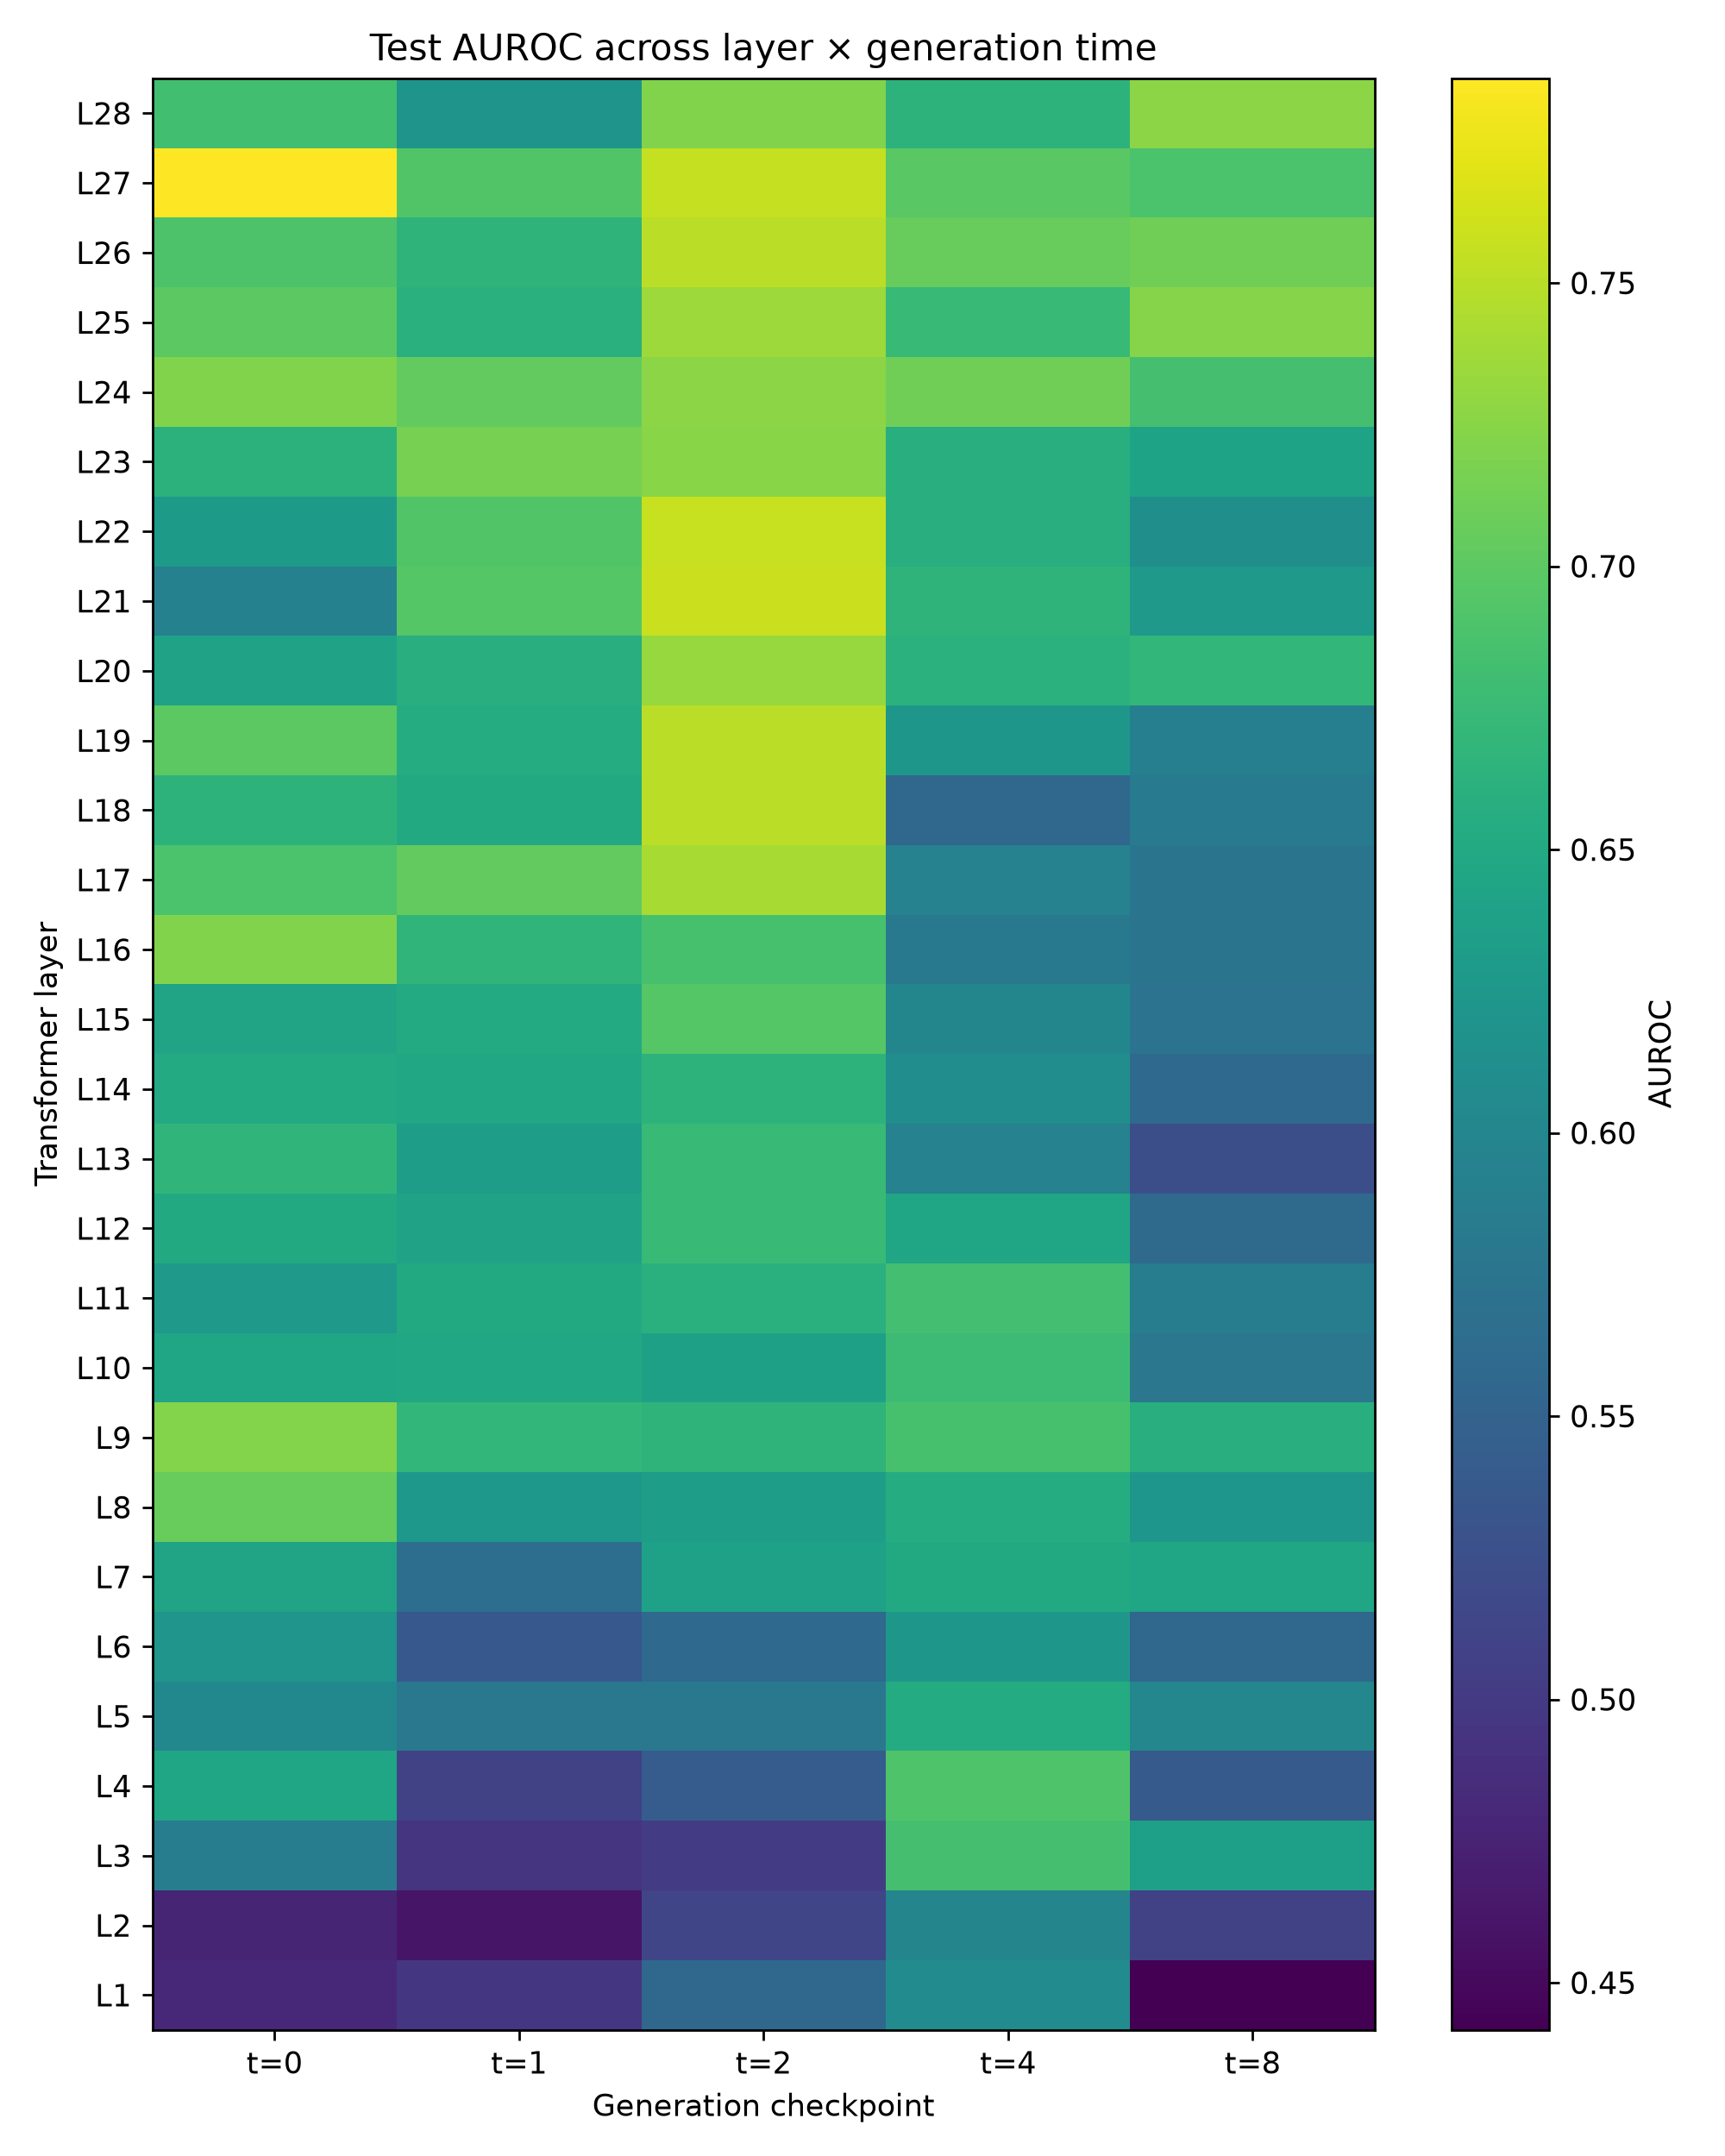
\includegraphics[width=0.72\linewidth]{results/step15_layer_time_test.png}
    \caption{Test AUROC of a simple probe at different transformer layers and generation checkpoints. Brighter regions indicate stronger correct-vs-hallucinated separability.}
    \label{fig:layer-time}
\end{figure}

The heatmap shows a clear qualitative pattern: later transformer layers generally contain stronger predictive signal than the earliest layers, especially around \(t=0\) and \(t=2\). The pattern is not monotonic over generation time. Later generated-token checkpoints do not simply become more informative.

This matches the early-detection result: the internal state before generation already carries substantial information, while later states appear to redistribute that signal rather than consistently strengthen it.

\section{Current Interpretation}

The experiments currently support the following interpretation.

\begin{enumerate}[leftmargin=1.6em]
    \item A factual failure can be predicted from internal representations before the first output token with AUROC around 0.80.
    \item The signal is not concentrated in one transformer layer. The best single-layer probe is weaker than models that combine information across layers.
    \item The strongest individual layer in the present validation split is Layer 20.
    \item A depth-aware GraphSAGE model gives a small average improvement over a flattened all-layer MLP and a shuffled-depth graph across five seeds.
    \item Full generation trajectories are not automatically better. In the current experiments, the \(t=0\)-only model performs better than models that include later generated-token states.
\end{enumerate}

The safest high-level conclusion is therefore:

\begin{quote}
\textit{Hallucination risk leaves a measurable, distributed internal signature across transformer depth before answer generation begins.}
\end{quote}

\section{What We Should Not Claim Yet}

The current experiments do not support claims such as:

\begin{itemize}[leftmargin=1.5em]
    \item ``The model knows that it will hallucinate.''
    \item ``Graph structure dramatically improves hallucination detection.''
    \item ``Layer 20 is the hallucination layer.''
    \item ``The method is already state of the art.''
\end{itemize}

The graph advantage is small, and the current study is based on one generator model and one main QA dataset. The strongest contribution at this stage is the analysis of \textit{when} and \textit{where} predictive information appears.

\section{Next Experiments}

The remaining experiments should focus on strengthening the analysis rather than adding a more complicated architecture:

\begin{itemize}[leftmargin=1.5em]
    \item paired uncertainty analysis for EpiGraph vs.\ MLP and shuffled GraphSAGE;
    \item depth-band analysis (early, middle, late layers) across generation checkpoints;
    \item answer-length and question-difficulty controls;
    \item replication on another QA dataset such as TriviaQA;
    \item optional replication with a second small language model;
    \item robustness to PCA dimensionality.
\end{itemize}

\section{Proposed Workshop Framing}

A suitable workshop framing is:

\begin{quote}
\textbf{When and where does a small language model internally reveal that a factual failure is likely?}
\end{quote}

EpiGraph can be presented as an analysis framework for tracing these internal signals across depth and generation time, rather than only as a classifier designed to maximize AUROC.

Possible working title:

\begin{center}
\textbf{Before the First Token: Tracing Epistemic Signals of Hallucination Across Transformer Depth and Generation}
\end{center}

\section{Repository Outputs Used in This Report}

The report summarizes the current outputs produced by the experimental pipeline, including:

\begin{itemize}[leftmargin=1.5em]
    \item \texttt{results/step07\_baselines.json}
    \item \texttt{results/step08\_epigraph\_sage.json}
    \item \texttt{results/step09\_shuffled\_sage\_seed42.json}
    \item \texttt{results/step10\_early\_detection\_seed42.csv}
    \item \texttt{results/step11\_t0\_all\_layer\_mlp\_seed42.json}
    \item \texttt{results/step12\_t0\_all\_baselines\_seed42.csv}
    \item \texttt{results/step13\_t0\_layerwise\_seed42.csv}
    \item \texttt{results/step14\_t0\_multiseed.csv}
    \item \texttt{results/step15\_layer\_time\_test.png}
\end{itemize}

\vfill
\begin{center}
\small
This document is intended as an internal research progress report and reflects the experiments completed so far.
\end{center}

\end{document}
